\chapter{The Growth of Functions}
\label{chap:growth}

\section{Introduction to Growth of Functions}
When analyzing computational complexity, evaluating an algorithm's performance on small inputs (e.g., $n = 5$ or $n = 10$) is deceptive. Modern processors execute billions of instructions per second, causing almost any elementary algorithm to terminate in imperceptible microseconds at small scales. 

Theoretical discrete mathematics focuses on the \textbf{rate of growth} of an algorithm's resource requirements as input size $n$ approaches infinity ($n \to \infty$). Section 3.2 of Rosen \cite{rosen2019discrete} establishes that the mathematical structure of the leading term completely dictates computational tractability.

\section{Importance of Input Size}
The parameter $n \in \mathbb{N}$ denotes the formal problem size (e.g., number of elements in an array, vertices in a graph, or bits in an integer). As $n$ grows, differences between complexity classes widen catastrophically.

\section{Hierarchy of Standard Growth Classes}
Rosen (§3.2, Table 1) \cite{rosen2019discrete} delineates the canonical complexity hierarchy:
\begin{equation}
\mathcal{O}(1) \prec \mathcal{O}(\log n) \prec \mathcal{O}(n) \prec \mathcal{O}(n \log n) \prec \mathcal{O}(n^2) \prec \mathcal{O}(2^n) \prec \mathcal{O}(n!)
\label{eq:hierarchy}
\end{equation}

\subsection{Constant Growth: $f(n) = 1$}
Execution demand is completely invariant to $n$. A constant-time algorithm executes identical instruction cycles regardless of whether $n = 10$ or $n = 10^9$. Typical examples include array indexing (\texttt{arr[k]}) and basic arithmetic operations.

\subsection{Logarithmic Growth: $f(n) = \log_2 n$}
Growth is exceptionally subdued. Doubling the input size $n \to 2n$ merely adds a constant $1$ to the function value:
$$\log_2(2n) = \log_2(2) + \log_2(n) = 1 + \log_2(n)$$
For an input of $n = 10^9$ elements, $\log_2(10^9) \approx 30$ operations. Typical example: Binary Search.

\subsection{Linear Growth: $f(n) = n$}
Resource consumption scales in direct proportion to problem size. Doubling $n$ doubles execution operations. Standard for single-pass sequential traversals (e.g., Linear Search).

\subsection{Linearithmic Growth: $f(n) = n \log_2 n$}
Slightly steeper than linear growth. Represents the proven information-theoretic lower bound $\Omega(n \log n)$ for general comparison-based sorting algorithms (e.g., Merge Sort, Heap Sort).

\subsection{Quadratic Growth: $f(n) = n^2$}
Resource consumption quadruples whenever input size doubles: $(2n)^2 = 4n^2$. Characteristic of nested pairwise element comparisons across sequences (e.g., Bubble Sort, Insertion Sort).

\subsection{Polynomial Growth: $f(n) = n^d$ ($d \ge 1$)}
Algorithms bounded by polynomial time $\mathcal{O}(n^d)$ are classified as computationally \emph{tractable} in complexity theory (the complexity class $\mathbf{P}$).

\subsection{Exponential Growth: $f(n) = 2^n$}
Each increment in input size $n \to n + 1$ doubles the computational burden. For $n = 64$, $2^{64} \approx 1.84 \times 10^{19}$ operations, requiring millennia of compute time on supercomputers.

\subsection{Factorial Growth: $f(n) = n!$}
Grows faster than exponential growth ($n! > 2^n$ for all $n \ge 4$). Characterizes brute-force permutation generators (e.g., Traveling Salesperson Problem).

\section{Comparison of Growth Rates}
Table \ref{tab:growth_functions} provides the exact numerical evaluation of these functions across selected discrete scales.

\begin{table}[htbp]
\centering
\caption{Numerical Evaluation of Standard Growth Functions (Rosen §3.2)}
\label{tab:growth_functions}
\small
\begin{tabular*}{\textwidth}{@{\extracolsep{\fill}}rrrrrrrr}
\toprule
$n$ & $\mathcal{O}(1)$ & $\mathcal{O}(\log_2 n)$ & $\mathcal{O}(n)$ & $\mathcal{O}(n \log_2 n)$ & $\mathcal{O}(n^2)$ & $\mathcal{O}(2^n)$ & $\mathcal{O}(n!)$ \\
\midrule
1 & 1 & 0.00 & 1 & 0.00 & 1 & 2 & 1 \\
2 & 1 & 1.00 & 2 & 2.00 & 4 & 4 & 2 \\
4 & 1 & 2.00 & 4 & 8.00 & 16 & 16 & 24 \\
8 & 1 & 3.00 & 8 & 24.00 & 64 & 256 & 40320 \\
16 & 1 & 4.00 & 16 & 64.00 & 256 & 65536 & 2.09e+13 \\
32 & 1 & 5.00 & 32 & 160.00 & 1024 & 4.29e+09 & inf \\
64 & 1 & 6.00 & 64 & 384.00 & 4096 & 1.84e+19 & inf \\
128 & 1 & 7.00 & 128 & 896.00 & 16384 & inf & inf \\
256 & 1 & 8.00 & 256 & 2048.00 & 65536 & inf & inf \\
512 & 1 & 9.00 & 512 & 4608.00 & 262144 & inf & inf \\
1024 & 1 & 10.00 & 1024 & 10240.00 & 1048576 & inf & inf \\
\bottomrule
\end{tabular*}
\end{table}


\section{Mathematical Interpretation of Growth Curves}
Figures \ref{fig:growth_common} and \ref{fig:growth_hierarchy} illustrate the mathematical growth functions generated through our analytical plotting pipeline.

\begin{figure}[htbp]
    \centering
    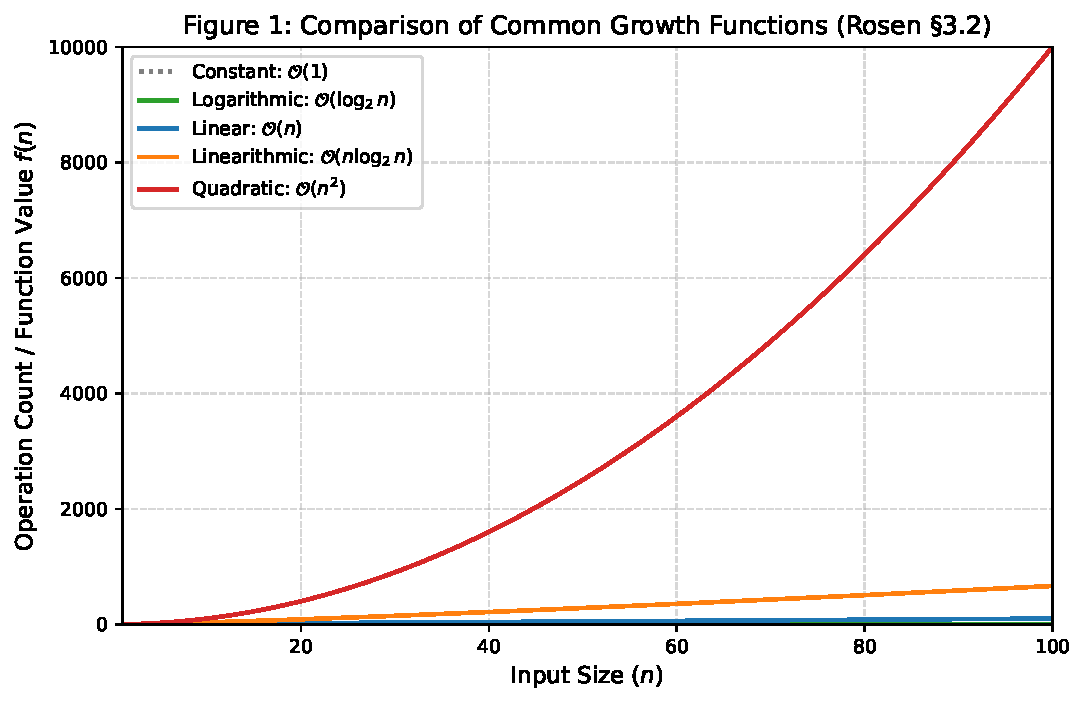
\includegraphics[width=0.88\textwidth]{latex/figures/figure1_common_growth_functions.pdf}
    \caption{Figure 1: Comparison of Common Growth Functions on Linear Scale (Rosen §3.2).}
    \label{fig:growth_common}
\end{figure}

\begin{figure}[htbp]
    \centering
    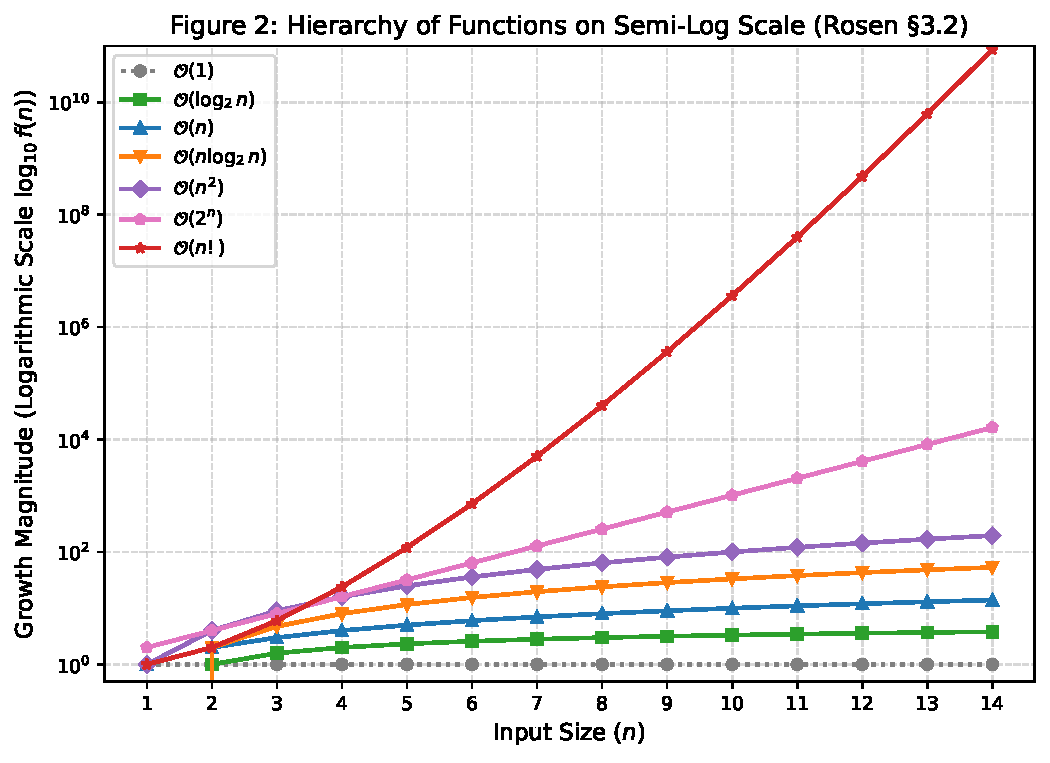
\includegraphics[width=0.88\textwidth]{latex/figures/figure2_growth_hierarchy_log_scale.pdf}
    \caption{Figure 2: Complete Complexity Hierarchy on Semi-Log Scale ($\log_{10} f(n)$) over $n \in [1, 14]$.}
    \label{fig:growth_hierarchy}
\end{figure}

Notice in Figure \ref{fig:growth_common} that on a linear scale, quadratic growth $\mathcal{O}(n^2)$ rapidly dwarfs linear and logarithmic curves. In Figure \ref{fig:growth_hierarchy}, when plotted on a logarithmic vertical scale, the exponential ($2^n$) and factorial ($n!$) curves skyrocket, establishing why intractable complexity classes cannot be rescued by hardware advancements.
